% Chapter 9

\chapter[Implementation]{Implementation} % Main chapter title

\label{Chapter9} % For referencing the chapter elsewhere, use \ref{Chapter9} 

%----------------------------------------------------------------------------------------

\section{Overview}
This section gives details of the implementation phase of the project, including descriptions of how parts of the system function, information regarding the development process and explanations for some of the key decisions made regarding the implementation.

The system was implemented closely following the design discussed in chapter \ref{Chapter8}, and is comprised of two parts; a full computer software application (referred to henceforth as `the application') and a collection of software classes and routines which form an `application programming interface' (API) and are designed to be included within the code a developer or researcher programs onto their robots. This API (referred to as the 'robot side code' or 'robot side API') presents the developer with functions to send data from the robot back to the application, and contains routines for handling the networking requirements to achieve this, and for correctly formatting the data. Both parts of the system implementation are fully independent. The application can be run on its own and receive data from another source, provided that this data correctly follows the format outlined in section \ref{DataTransferFormat}. The application is the much larger of the two system parts, and therefore will be the focus of the majority of this implementation chapter. 

Figure \ref{fig:UI} shows the user interface for the application as it is seen at start-up, and can be compared to figure \ref{fig:UILayout} in chapter \ref{Chapter8} to relate it with the user interface design. The key features of the application can be seen in this image. This includes the video feed augmented with information about the three visible robots, including position, direction, ID number, and for the selected robot name and current state. The robot list panel is also visible on the right hand side, showing the IDs and names of the known robots, and which is currently selected. Finally the data panel can be seen at the bottom of the application, currently set to the overview tab, providing more detailed information about the selected robot.

\begin{figure}
	\centering
	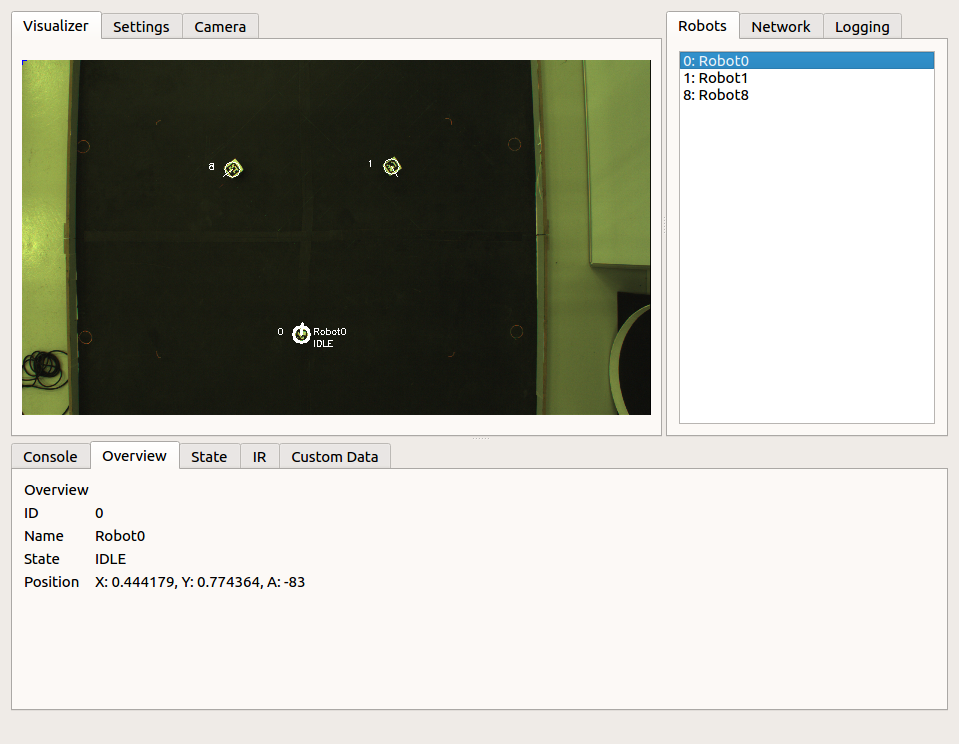
\includegraphics[scale=0.4]{Figures/ApplicationScreenshotOverview.png}
	\decoRule
	\caption[Application User Interface]{The user interface for the application.}
	\label{fig:UI}
\end{figure}

The Qt application programming framework was used to organise the application implementation and provide the user interface components, as well some lower level functionalities such as threading and timers.

%----------------------------------------------------------------------------------------

\section{Code Structure}
The code files for the system exist in two groups; a collection of C++ source and header files which make up the main application, and a smaller collection of C++ source and header files which handle the robot-side portion of the system. In addition to the source files the main application also relies on a number of other files which are used by the Qt system to define the user interface and manage the build process. Table \ref{tab:CodeFiles} details the names and purposes of all files within the main application. Table \ref{tab:RobotCodeFiles} details the files that make up the robot side API.

\begin{longtable}{ l p{10cm} }
\caption[Application Code Files]{Source code and tertiary files that make up the main application.}\\
 File & Purpose\\ 
 \hline
 main.cpp & The entry point for the application. Instantiates the MainWindow class.\\
 mainwindow.cpp, .h & The core class, contains the entry point for the application and controls the set up and tear down processes and handles UI events within the main window.\\
 mainwindow.ui & Describes the user interface layout in a XML-like format. Used by the Qt framework to construct the UI.\\
 datamodel.cpp, .h & The top level class encapsulating the full data model. Maintains a list of RobotData objects.\\
 robotdata.cpp, .h & A class encapsulating the data of a single robot, including ID, position, state, sensor data and user data.\\
 datathread.cpp, .h & This class contains all routines for receiving data from the robots via wifi, and is designed to be run on a thread of its own.\\
 cameracontroller.cpp, .h & The high level class encapsulating the routines and data related to the tracking camera. This class is designed to be independent of the camera hardware being used.\\
 machinevision.cpp, .h & A lower level class encapsulating routines for interfacing with the camera hardware.\\
 visualiser.cpp, .h & This class encapsulates the visualiser GUI object, and is implemented to conform the Qt framework as a custom extension to the QWidget class. Also contains routines for applying the video augmentations as per the current visualiser settings.\\
 viselement.h & Contains an abstract class definition for a single visualiser settings element. These elements are used to define how specific elements of the video augmentation are rendered, and also contain settings and variables relevant to this task. \\
 vis*.cpp, .h, .c & Classes beginning with the `\textit{vis}' prefix derive from the VisElement abstract class and contain routines for rendering the visualisation for one type of data. The latter part of the class name identifies which data type is targeted.\\
 irdataview.cpp, .h & A custom GUI object, derived from QWidget, which displays the raw IR sensor data as a bar graph in the data window.\\
 settings.cpp, .h & Encapsulates the general application settings and routines for changing their values according to user input.\\
 log.cpp, .h & Encapsulates the routines for logging events and data to text files.\\
 util.cpp, .h & Contains static utility functions used in various places throughout the application code.\\
 *settingsdialog.cpp, .h & Classes ending with the `\textit{settingsdialog}' suffix describe dialog windows for adjusting the settings related to the visualisation of specific data types, identified by the first part of the class name.\\
 appconfig.h & Contains pre-processor definitions for controlling inclusion/exclusion of code segments.\\
 SwarmDebug.pro & Used by the Qt framework to build the application. Directs to the necessary code files and libraries.\\
 \bottomrule\\
	
 \label{tab:CodeFiles}
\end{longtable}

\begin{longtable}{ l p{10cm} }
\caption[Robot-side Code Files]{Source code files that make up the robot side API.}\\
 File & Purpose\\
 \hline
 debug\_network.cpp & This file encapsulates networking functionality for communicating with the debugging system. Contains routines for sending data of specific types, as well as for sending raw packets.\\
 debug\_network.h & Header file for the debugging system network interface. Also contains definitions for data type identifiers.\\
 \bottomrule\\
	
 \label{tab:RobotCodeFiles}
\end{longtable}

%----------------------------------------------------------------------------------------

\section{Video Feed and Tracking System} \label{VideoFeedAndTrackingSystem}
The code relating to retrieving images from the machine vision camera and running the ARuCo tag tracking algorithm can be found in the files \textit{cameracontroller.cpp / .h} and \textit{machinevision.cpp / .h}. This code is run on the separate camera thread, in order to maximise application performance and ensure responsiveness in the event that the camera driver blocks execution whilst retrieving the next frame. The \textit{CameraController} class handles the higher level operations such as running a timer to periodically poll the camera driver for the next image, supplying the driver with the correct dimensions for the image to be resized to in order to fit within the available space in the UI, and converting the image itself and the tracking data into formats which can be passed back to the main thread and used in the UI and data model respectively. The application threading is handled through the use of the Qt framework's \textit{QThread} API, and communication between threads utilises the framework's `\textit{signals} and \textit{slots}' feature, which allows components on different threads to send and receive data in a managed, thread-safe manner. The \textit{CameraController} class therefore utilises two signals; one for emitting the camera image data, and another for emitting the robot position data. At initialisation time the application's core class, \textit{MainWindow}, connects these signals to matching slots within the \textit{Visualiser} and \textit{DataModel} classes respectively.

The \textit{MachineVision} class handles the lower level operations related to the camera and the tracking system, including setting up the camera driver, retrieving and resizing individual images from the camera and running the ARuCo tag detection algorithm. For each tag detected in the image the ARuCo algorithm returns the pixel coordinates of the four corners of the tag. The \textit{MachineVision} class includes code to average out these four coordinates to get a center point, and then convert this pixel coordinate to a 'proportional' coordinate; two numbers between 0 and 1 which represent the horizontal and vertical components of the position as a proportion of the full height and width of the image respectively. This ensures that the robot positions can still be correctly displayed after the image has been resized, without having to maintain information related to the resizing operation.

%----------------------------------------------------------------------------------------

\section{Networking}
The networking requirements of the system were relatively simple, and can be summarised as follows:

\begin{enumerate}
	\item Must utilize a WiFi network.
	\item Must allow a large number of sources to transmit data to a single host
	\item Must allow for frequent transmission of small packets of data
\end{enumerate}

WiFi networks utilise the standard Internet Protocol (IP) network layer protocol. There are two commonly supported transport layer protocols which run on top of IP, the Transmission Control Protocol (TCP) and the User Datagram Protocol (UDP). TCP is a managed and delivery-error checked protocol, and therefore guarantees that packets will be transmitted in the correct order, with lost packets being retransmitted. This adds overheads such as acknowledgements to the protocol, and requires an established 'connection' in order to function correctly. TCP also operates a queueing system, whereby packets for transmission are held until a number of them are ready, and can therefore be grouped together and sent. UDP, by contrast, does not error check the delivery of packets, making no guarantees that a packet will be received, or that packets will be received in the correct order, removing the need for an established connection and reducing the overheads involved. Packets can therefore be sent from any application to any target IP address and port on the network, without first establishing a connection with another application. Packets are also sent immediately, with no queueing system in place It was determined that the User Datagram Protocol (UDP) would be the most suitable for this system, for a number of reasons. The connection requirements of TCP would require the to form a connection with application each robot prior to transmitting data, which would add unnecessary complexity. Using UDP also ensured that the packets were transmitted immediately, reducing the potential for latency in the system. The lack of delivery checking was not considered an issue, as the robots would be transmitting updates frequently enough that a single lost packet would not cause a significant issue.

Code relating to the networking functionalities of the application is contained in the files \textit{datathread.cpp / .h}, which encapsulate the \textit{DataThread} class. This class is run on a dedicated thread to ensure that potentially blocking operations do not impact application performance. This class contains routines for dealing with the low level network requirements, such as establishing a socket through which to receive data packets from the robots, and continually listening on this socket for new data. All socket operations are implemented using structures and definitions from the standard C++ networking libraries. Data received from the robots is passed to the main application thread through a Qt signal, using the Qt signals and slots interface in the same manner as described in section \ref{VideoFeedAndTrackingSystem}. The main application class, \textit{MainWindow}, connects this signal to the appropriate slot in the \textit{DataModel} class. The application side networking is configured in the \textit{network} tab of the right-hand panel of the user interface. The user is able to enter a desired port number on which to receive data, and can begin listening for packets on this port by pressing the `\textit{start listening}' button.

Within the robot side API, the networking functionality is implemented in a very similar way. The initialisation function establishes a target socket based on a supplied IP address and port. This should match the IP address of the computer or server running the main application, and the port chosen by the user within the main application. When any of the functions for sending specific data packets are called, the data is then sent to this target socket. All socket operations are again implemented using the standard C++ networking libraries.

%----------------------------------------------------------------------------------------

\section{Data Transfer Format} \label{DataTransferFormat}
In order to retrieve data from the robots in a usable fashion a common format for exchanging data needed to be defined, and used by both ends of the communication link. A number of different options were considered for achieving this, ranging from super-lightweight custom packets using the minimum number of bytes to established existing solutions such as the JSON data interchange standard. The primary concerns when making this decision were a desire to minimise any overhead in terms of extra code needed on the robot side, as the robots have limited memory, and to ensure the format remained as simple as possible, so that future extensions to the system, such as implementations for other robots, could be programmed with relative ease. It was ultimately decided not to use JSON, to avoid the need for any additional code libraries to be stored in the robot's memory, and to instead use a custom simple string-based packet format. All data to be transmitted from the robot to the application is therefore converted to a simple string which is then transmitted in the data packet. As well as containing the data, the string must identify the robot and describe the type of data within. The format for these strings was defined as

\begin{center}
[ROBOT ID] [PACKET TYPE] [DATA]
\end{center}

%----------------------------------------------------------------------------------------

\section{Data Model}


%----------------------------------------------------------------------------------------

\section{Visualiser}


%----------------------------------------------------------------------------------------

\section{User Interface}


%----------------------------------------------------------------------------------------

\section{Robot Code}


%----------------------------------------------------------------------------------------